\documentclass[11pt]{article}
\usepackage{makecell}
\usepackage{amsfonts}
\usepackage{amsmath}

\usepackage{MyTemplate}

\usepackage{endnotes}

\let\footnote=\endnote

\newcommand{\پاورقی}[1]{\footnote{\lr{#1}}}
\newcommand{\cols}[1]{
 \begin{tabular}{@{}c@{}} #1 \end{tabular}
}   


\begin{document}

\thispagestyle{empty}
\begin{center}

\includegraphics{logo}
\vskip 1cm

\large{
{\bf
دانشگاه صنعتی شریف\\ دانشکده مهندسی کامپیوتر\\ سمینار کارشناسی ارشد گرایش هوش مصنوعی
}
\\
\vskip 1cm
عنوان:\\
{ \bf
تست تست
}
\\{ \bf \large
\lr{ My test }}
\vskip 1cm
نگارش:\\
\textbf{امیر پورمند}
\\
\vskip 0.5cm
شماره دانشجویی: \\
3123123123213
\\
\vskip 1cm
استاد راهنما:\\
 \textbf{دکتر  }
 \\
\vskip 1cm
استاد ممتحن داخلی:\\
\textbf{دکتر  }
\\

\vskip 3.5cm

}
بهمن ۱۴۰۰
\newpage
\end{center}





{\bf {چکيده: }}
روش‌های تشخیص پولیپ به کمک کامپیوتر تأثیر زیادی در کم کردن نرخ عدم تشخیص 

{\bf  { واژه‌های کلیدی: }}
تشخیص پولیپ، دسته‌بندی پولیپ، سرطان روده، کولونوسکوپی، تشخیص بی‌درنگ

\setlength{\parindent}{0.25in} %The indent of the paragraph first line

\section{مقدمه}
امروزه سرطان یکی از مهم‌ترین بیماری‌هایی است که سلامتی افراد را تحت تاثیر قرار داده است و همچنین نرخ مرگ و میر بالایی نیز دارد. سرطان‌ها بر اساس تومور بدخیم پدید می‌آیند. در تمام انواع سرطان، بعضی سلول‌ها تقسیم می‌شوند و در اطراف پخش می‌شوند
\cite{pacal2020comprehensive}.
سرطان روده سومین عامل مرگ و میر در جهان در بین مردان و دومین عامل مرگ در بین زنان است. 
به طور کلی ریسک گرفتن سرطان روده برای مردان 
$4.3$ \%
و برای زنان 
$4.0$ \%
است
\cite{cancer_keystatistics}.



\section{واژگان تخصصی تحقیق (اختیاری)}

\paragraph{پولیپ (\lr{Polyp})}
به صورت رشد غیرطبیعی توده‌های خوش‌خیم در جدار اعضای بدن تعریف می‌شود؛ مانند پولیپ روده، معده، بینی و پولیپ رحم.
\textbf{پولیپ، سرطان نیست}
ولی سرطان می‌تواند منشا آن باشد. 
پولیپ می‌تواند در هر جایی ظاهر شود ولی معمولا در ناحیه روده ظاهر می‌شوند
\cite{Jha_2021}.
%% Todo: انواع پولیپ 
پولیپ به طور کلی در دو دسته نئوپلاستیک
\lr{(neoplastic)}
و غیر نئوپلاستیک
\lr{(non-neoplastic)}
دسته بندی می‌شود. پولیپ‌‌های غیرنئوپلاستیک معمولا سرطانی نیستند و خطری ندارند. این پولیپ‌ها به سه زیردسته هایپرپلاستیک 
\lr{(hyper-plastic)}
،
التهابی 
\lr{(inflammatory)}
، 
همارتوماتوز
\lr{(hamartomatous)}
تقسیم بندی می‌شوند. در سوی دیگر پولیپ‌های نئوپلاستیک هستند که می‌توانند به پولیپ سرطانی تبدیل شوند. این پولیپ‌ها نیز به دو زیردسته 
آدنوما
\lr{(adenomas)}
و
دندانه‌دار 
\lr{(serrated)}
تقسیم‌بندی می‌شوند
\cite{Jha_2021}.


\paragraph{کولونوسکوپی 
	(
	\lr{Colonoscopy}
	)
} 
آزمایشی است که برای تشخیص تغییرات یا موارد غیر عادی در روده بزرگ و رکتوم (راست روده) مورد استفاده قرار می گیرد.
در طول کولونوسکوپی یک لوله طولانی و انعطاف پذیر به نام کولونوسکوپ داخل رکتوم (راست روده) قرار داده می شود. یک دوربین ویدئویی کوچک در بالای لوله وجود دارد که به پزشک اجازه می دهد تا داخل کل روده بزرگ را به خوبی مشاهده کند. در طول کولونوسکوپی، اگر نیاز باشد، پولیپ یا سایر بافت های غیر طبیعی را می توان حذف کرد. 




\section{ادبیات پژوهش}



در  مقالات اکثرا از روش‌های مبتنی بر CNN 
استفاده شده که روش‌ حل ما نیز بر اساس همان است. شبکه‌های استفاده شده در مقالات 
\lr{R-CNN}
، 
\lr{Fast R-CNN}
،
\lr{Faster R-CNN}
و
\lr{YOLO}
بوده است. 




به طور کلی روش‌های تشخیص شی دو دسته هستند
\cite{zaidi2021survey}:

\begin{itemize}
	\item
	روش های مبتنی بر پردازش تصویر که ویژگی‌ها را بصورت دستی استخراج می‌کنند ولی نیاز به داده برچسب‌دار ندارند. عیب اصلی این روش‌ها این است که در مواجهه با سناریوهای پیچیده‌تر مثل استتار
	\پاورقی{occlusion}
	کارا نیستند. 
	\item
	روش‌های مبتنی بر یادگیری عمیق که 
	مبتنی بر یادگیری تقویتی هستند و کارایی آن به قدرت GPU که روی آن پردازش می‌شود نیز بستگی دارد. 
	این روش‌ها در مواجهه با سناریوهای پیچیده‌تر مثل استتار
	و یا نوردهی متفاوت
	\پاورقی{illumination}
	کاراتر هستند ولی نیاز به داده برچسب‌دهی شده زیادی دارند. 
\end{itemize}

روش‌های مبتنی بر یادگیری عمیق نیز به دو دسته کلی تک مرحله‌ای
\پاورقی{single-stage}
و دومرحله‌ای
\پاورقی{multi-stage}
تقسیم بندی می‌شوند که در ادامه آن‌ها را به تفضیل بررسی خواهیم کرد. 
پیش از این توجه داریم که
با توجه به این که روش‌های مبتنی بر پردازش تصویر نمی‌توانند ساختارهای پیچیده‌تر را یاد بگیرند و عموما دقت کمی دارند در این تحقیق بر روی روش‌های مبتنی بر یادگیری عمیق متمرکز خواهیم شد.


\subsection{روش های دومرحله‌ای}

\subsubsection{R-CNN}

مدل 
\lr{R-CNN}
\cite{girshick2014rich}
در سال ۲۰۱۴
معرفی شد که برای هر تصویر سه مرحله را انجام می‌هد. در این الگوریتم (همان طور که در شکل 
\ref{fig:rcnn}
نشان داده شده است
)، ابتدا با استفاده از یک الگوریتم پیشنهاد ناحیه
\lr{(region proposal)}
به نام جستجوی انتخابی
\lr{(selective search)}
تعدادی (تقریبا ۲۰۰۰ تا) ناحیه استخراج می‌شود، سپس نواحی استخراجی از یک شبکه CNN عبور می‌کند و با استفاده از SVM
\پاورقی {
	\lr{Support Vector Machine}
}
دسته‌بندی انجام می‌شود. 

اهمیت این شبکه از این لحاظ است که از مدل‌های پیشین خود به طرز شگفت آوری بهتر عمل کرد و mAP را ۳۰ درصد افزایش داد. معایب این روش این است که آموزش شبکه بصورت انتها به انتها انجام نمیشود و یک فرآیند چندمرحله‌ای داریم که باعث کند شدن سرعت شده است. ثانیا آموزش این مدل هم از نظر زمانی و هم از نظر فضای دیسک بسیار هزینه بر است زیرا ویژگی‌ها به ازای هر تصویر استحراج می‌شوند و بر روی دیسک نوشته می‌شوند که باعث اشغال کردن مقدار زیادی فضا می‌شود (در حد چند صد گیگابایت. 

% TODO: \usepackage{graphicx} required
\begin{figure}
	\centering
	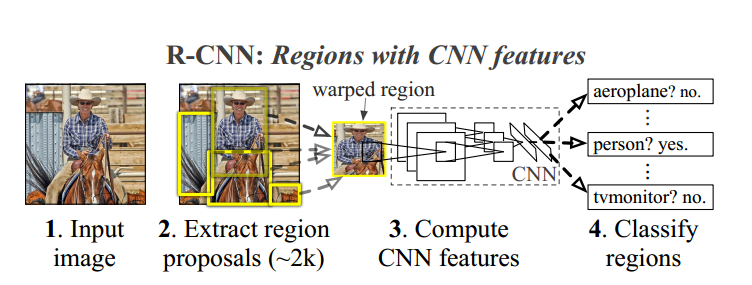
\includegraphics[width=0.7\linewidth]{images/rcnn}
	\caption[خلاصه مراحل تشخیص در R-CNN]{}
	\label{fig:rcnn}
\end{figure}




\subsection[تشخیص و دسته‌بندی پولیپ] {تشخیص  و دسته‌بندی پولیپ \پاورقی{Polyp detection and classification}}

نیز در زمره بهترین معماری‌های یادگیری عمیق قرار دارند. در جدول مقایسه
 کاملی بین روش‌های قبلی در این زمینه وجود دارد. همان طور که مشخص است تعداد کارهای انجام شده ای که هم تشخیص و هم دسته‌بندی پولیپ را انجام دهند بسیار کم است و در چند سال گذشته نیز کسی روی این زمینه کار نکرده است.



\clearpage
\section{آزمایش‌های اجرا شده}
 
\begin{table}[]
\centering
\caption{مجموعه دادگان مورد استفاده در پژوهش}
\label{tab:datasets}
\begin{tabular}{cccc}
\hline
مجموعه دادگان       & تعداد تصویر یا ویدئو & رزولوشن                                     & کار               \\ \hline
\lr{CVC-ClinicDB}        & 612 تصویر            & SD
،
$384 \times 288$  & تشخیص و مکان‌یابی \\ \hline
\lr{CVC-VideoClinicDB}   & 18 ویدئو             & SD
، $768 \times 576$  & تشخیص و مکان‌یابی \\ \hline
\lr{Colonoscopy Dataset} & 76 ویدئو             & SD
، $768 \times 576$  & دسته بندی         \\ \hline
\lr{ETIS-Larib}          & 196 تصویر            & HD
، $1225 \times 966$ & تشخیص و مکان‌یابی \\ \hline
\lr{Kvasir-SEG}          & 1000 تصویر           & متفاوت                                      & قطعه‌بندی  
%\\ \hline
%\lr{Kvasir} & & & \\ \hline
%\lr{Hyper-Kvasir} & & & 
\end{tabular}

\end{table}

\linespread{1}
\small
\setlength{\parskip}{0pt}
\setlength{\parsep}{0pt}
%\Latin
\pagebreak
\clearpage
\renewcommand{\refname}{\rl{{مراجع}\hfill}}
\begin{latin}
\baselineskip=.9\baselineskip
\bibliographystyle{unsrtabbrv}
\bibliography{ref}
\end{latin}

\newpage




%\Persian
\section*{واژه‌نامه}
\begin{LTR}
\begin{multicols}{3}
\LTRmulticolcolumns
\theendnotes 
\end{multicols}
\end{LTR}
\end{document}

